\newcommand{\package}{\emph}
\chapter{Introduction}
Solar energy is one of the key alternative energy sources. The recent developments in solar panels and different business models around them made the photo-voltaic(PV) power plants more economical. However, the fluctuation in PV output power make the integration into main energy grid risky and slow. These fluctuation comes from cloud states in sky, and it has two different effects, one decreasing the power, the other one increasing the power. Firstly, if the clouds cover the sun completely or partially, some area of plant is shaded and does not receive direct sunlight, causing a power drop. On the other hand, if the clouds are not blocking the the sun completely or at all, based on their type, height, position and time, they can re-reflect some part of the irradiation\footnote{Irradiation is the sum of irradiance over a time period, expressed in  $Wh/m^2$} which is reflected by ground, back into the power plant. In this case, the input irradiance\footnote{Irradiance is understood as instantaneous density of solar radiation incident on a given surface, typically expressed in $W/m^2$} and consequently the output power increases. In the electricity grid, the stability of power is vital. Therefore, if we want to integrate a PV power source into the grid we need to compensate for any power drop by using other electricity sources, and also restrain any excessive power. That is why we need to predict these short-time power changes in advance to design better strategies for handling them and ultimately provide a guaranteed stable power in the grid. In this chapter, we first explain different approaches towards this prediction problem, then we describe overview of the setup used in this study, and finally we talk about challenges in this setup and  accuracy measures for the result. 


\section{Power prediction approaches for a PV plant}
\label{sec:overview}
The approaches which are used in weather forecast applications deal with prediction of long term irradiance patterns, however, for power prediction applications we are mostly interested in very short-time prediction which stretches up to one hour ahead. Since the movement of clouds and their shape is so dynamic that makes the longer predictions infeasible. Even though, there are some studies focusing on pattern recognition of meteorological data for irradiance prediction, in this study we focus on vision-based methods which seem to be more accurate and inexpensive.
\subsection{Satellite-based imagery}
There are some methods using live feed of satellite images from the area on top and around PV plant for determining cloud movements and estimating their position in a specific time in the future assuming the constant velocity and fixed direction model. Then by using the geometrical parameters including cloud height and the plant area, they project the clouds onto the plant area in order to determine shaded areas.
%\subsection{Several irradiance sensors in ground}

\subsection{Ground whole-sky imagery}
The second approach is using the image sequence of a sky-facing camera which is located in the PV plant site. In this context, movement of clouds are identified by analyzing the consecrative image frames and then projected into a specific time in future using fixed velocity vector model. For the next step, some methods project the clouds into the ground and determine shaded parts of the plant. In order to obtain high accuracy on shadow mapping, knowing the cloud height is very important. Therefore, some methods use an specific laser sensor to get the cloud base height at any given time. It is also possible to use two cameras in the site mounted with a distance and by applying stereo algorithm, find the cloud height; however, this method has not been investigated in practice yet.

\section{Data acquisition setup}
This study uses the data from a PV plant in Cavriglia area in Italy.
The setup for this study is based on one fish-eye camera mounted at the top of the building right next to the PV plant. This type of camera with 180 degree area of view gives us the whole sky in one image. Furthermore, there are two irradiance sensors located at the same location as camera, one with the same angle as solar panels-which is tilted towards the south- and the other one about 40 degrees tilted towards the north. The data acquisition software takes several images with different exposures every 6 seconds and combine them to get HDR images. The irradiance sensor measurements and temperature are also recorded at the same intervals. Finally, we record power output of PV plant every 3 seconds.

\section{Cloud segmentation, cloud tracking}
For predicting the future state of clouds in the sky we need to first know where are the clouds. This is done by applying a dynamic-threshold segmentation algorithm on red to blue channel ratio of RGB images. Several studies has shown that the red to blue ratio is a good criterion for cloud segmentation, but the threshold for this ratio should be set in a way that discriminate clouds locally but be smooth globally. This method handles cloud color variation on different cloud types very well. One sample result of such segmentation is figure \ref{fig:cloud_seg}
\begin{figure}[h]
\caption{Cloud segmentation sample}
\label{fig:cloud_seg}
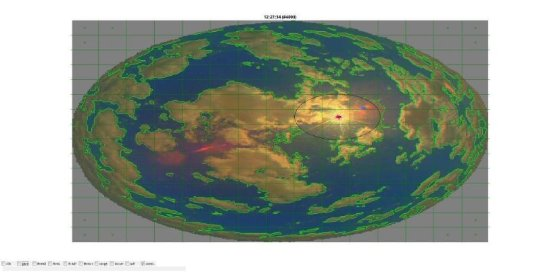
\includegraphics[scale=.6]{cloud_segment}
\centering
\end{figure}

After detecting the clouds in a sequence of images, one can apply optical flow algorithm on some points of interest in the first image and extract the cloud movement as motion vectors of optical flow. This cloud tracking pipeline gives us the clouds position is the sky for very short time in future. The result of experiment on several future time horizon has shown that accuracy decreases considerably after 30 minutes, specially in high speed cloud motions.

\section{Image irradiance estimation for power prediction}
The final step in power prediction is to associate a potential power estimate to any time in several minutes ahead knowing the cloud positions and their characteristic in that time. The generated power of a PV plant depends on several factors including received irradiance, operational temperature and panels specification. However, the only factor which changes rapidly and has a huge impact on the output power is irradiance. Therefore, in our power prediction framework, we use a power prediction adaptation method with recorded data of previous minutes to derive the power output from future irradiance estimations. The scaling factor for the result is calculated by diving the recorded power output and irradiance sensor measurements. Thus, this power adaptation mechanism, separates and defines our main problem as estimating the received irradiance from a clouds attributes in a specific time and location.

\section{Irradiance components}
The total solar radiation -GHI\footnote{Global Horizontal Irradiation}- which hits the surface of solar panels consists of three basic components, direct -DNI\footnote{Direct Normal Irradiance}-, diffuse -DHI\footnote{Diffuse Horizontal Irradiance}- and reflected. The direct part comes from the sunlight beams directly raying from sun direction to the solar module. While passing through atmosphere, some amount of sunlight scatters in every direction by dense particles. The portion of this scattered light which hits the module forms the diffuse irradiation for solar panels. 
Reflected irradiance represents sunlight that is reflected off the clouds or ground around the array of panels. The source of this reflected radiation can be DNI or DHI. Rate of the reflection depends on clouds coverage, size of the ground that is visible from the module and their albedo coefficient\footnote{The portion of the incident irradiance that is reflected}. The albedo coefficient for ground is typically 0.2, though it can be higher during snowy periods in cold climates. The albedo coefficient for clouds depends on their type, density, temperature and etc. These components are shown in figure 	\ref{fig:irr_comps}

\begin{figure}[h]
\caption{Irradiance components}
\label{fig:irr_comps}
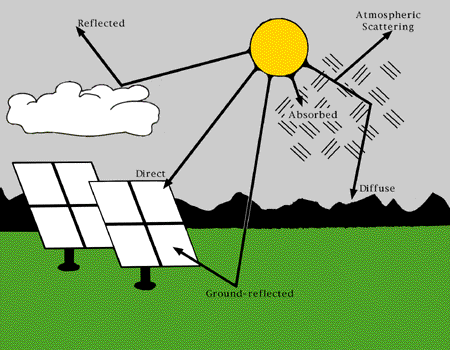
\includegraphics[scale=.7]{irr_components}
\centering
\end{figure} 

Total irradiation is related to other three components with this formula:
\[ GHI = DNI \times cos (Z) + DHI + reflected \]
where Z is the solar zenith angle-the angle between the direction of the sun and the line directly overhead.
Since distinguishing between the reflected and diffuse irradiation is practically hard and also there is not any ground truth value for training, we decided to combine both of them as the diffuse component. Thus, the formula changes to:
\begin{equation}
GHI = DNI \times cos (Z) + DHI
\end{equation}
where DHI is sum of all non direct irradiations.
\section{Accuracy metrics}
For measuring accuracy of the result we can use popular error measures such as RMSE-Root mean square error. However, since there are not any other publicly available study on this specific problem to compare our RMSE with, we can define our own error measures which quantify our solution quality better. For example, apart from RMSE, we calculate a relative error as well that penalize errors for irradiances higher than a specific value more. And errors for irradiances lower than that value, will be penalized less. This cutting value is set as 100 and the scale is logarithmic, because when the irradiance is less than 100, the power output of plant is very low and practically not useful in grid. On the other hand, we want more precise result for very high irradiances. This means errors for small irradiances are less important than errors in big big ones. We also use MBE (mean bias error) and $R^2$ for correlation coefficient.
%\section{Challenges}


